\subsection{Results} \label{Sec:results}
\headbf{Accuracy (RQ1)}
\tabref{accuracyTable} shows the number of  correctly reported (true positive), the number of incorrect reported (false positive), and the number of missed (false negative) \javascript lines of code, as well as precision and recall achieved by \tool, which are related to human-written DOM-based assertions. The table also shows the number of explicit, implicit, candidate, and the total number of assertions generated by \tool. The recall achieved for Phormer (ID 1), WolfCMS (ID 3), and AddressBook (ID 6) is 100\%. For EnterpriseStore (ID 2), Claroline (ID 4), and StudyRoom (ID 5) the recall achieved is 84\%, 79\%, and 82\% respectively. Except for EnterpriseStore and Claroline applications, for which the precision rate is 98\%, the computed precision rate for the rest of applications is 100\%.

We noticed that the lower recall rate obtained by \tool is mainly due to the use of third party libraries. Currently, we only analyze the application source code and do not consider libraries in our slicing technique. The underlying assumption is that faults mainly originate from the application's code. The small drop observed in precision is due to functions that are called but not instrumented due to limitations in our current implementation. If the definition of a called function is not instrumented, we assume that the function call is related to our slice, while it may not be so. 
We also observed that in rare cases a variable is seemingly assigned by a return value of a function, though the \code{return} statement is not found in the body of the called function. Our current implementation includes such variable assignments in the pertaining slices. 
Note that both recall and precision can be improved to 100\% with a more robust implementation of our technique. 

We found out that on average 6\% of the human-written DOM-based assertions in our experimental objects are not connected to the \javascript code in the following scenarios: (1) HTML is used to transfer the data, which is required by the client from the server (e.g;, the required information is stored as meta-data in attributes within the HTML), (2) web server is utilized to perform computations, (3) instead of dynamically generating the DOM structure through the \javascript code, HTML fragments are retrieved from the server and injected into the page, and (4) CSS and HTML are used to perform required changes to the user interface (e.g.; the CSS transition property with \code{hover} is used to bypass \javascript).
\begin{table}
        \caption{Accuracy achieved by \tool.} \label{Table:accuracyTable}        
{\scriptsize
\centering
%    \begin{center}
       
      %  \subtable[Experimental subjects and the corresponding exploration data]
            {
           \begin{tabular}{c|c|c|c|c|c||c|c|c|c} \hline
           
&\multicolumn{5}{c||}{\thead{Backward Slice}} & \multicolumn{4}{c}{\thead{Assertions}} \\
\cline{2-10}
          
           
           
\theadturn{App ID} &\theadturn{\# TP (LOC)} &\theadturn{\# FP (LOC)} &\theadturn{\# FN (LOC)} &\theadturn{Precision (\%)} &\theadturn{Recall (\%)} & \theadturn{\# Explicit} & \theadturn{\# Implicit} & \theadturn{\# Candidate} &\theadturn{\# Total}  \\  \hline 
\hline 
1  & 174 & 0 & 0 & 100 & 100 & 41 & 9 & 13 & 63     \\ \hline
           
2 & 861 & 18 & 162 & 98 & 84 & 51 & 19 & 26 & 96    \\ \hline

3 & 193 & 0 & 0 & 100 & 100 & 83 & 23 & 16 & 122   \\ \hline

4 & 1446 & 29 & 385 & 98 & 79 & 72 & 29 & 31 & 132\\ \hline

5 & 1017 & 0 & 224 & 100 & 82 & 78 & 18 & 11 & 107  \\ \hline

6 & 533 & 0 & 0 & 100 & 100 & 24 & 3 & 14 & 41  \\ \hline

7 & 430 & 0 & 0 & 100 & 100 & 14 & 5 & 16 & 35  \\ \hline

AVG & - & - & - & 99.4 & 92.1 & - & - & - & - \\ \hline
\hline\end{tabular}
            }

%\end{center}
}
%\vspace{-0.2in} 
\end{table}
\begin{figure}[!t]
  \centering
  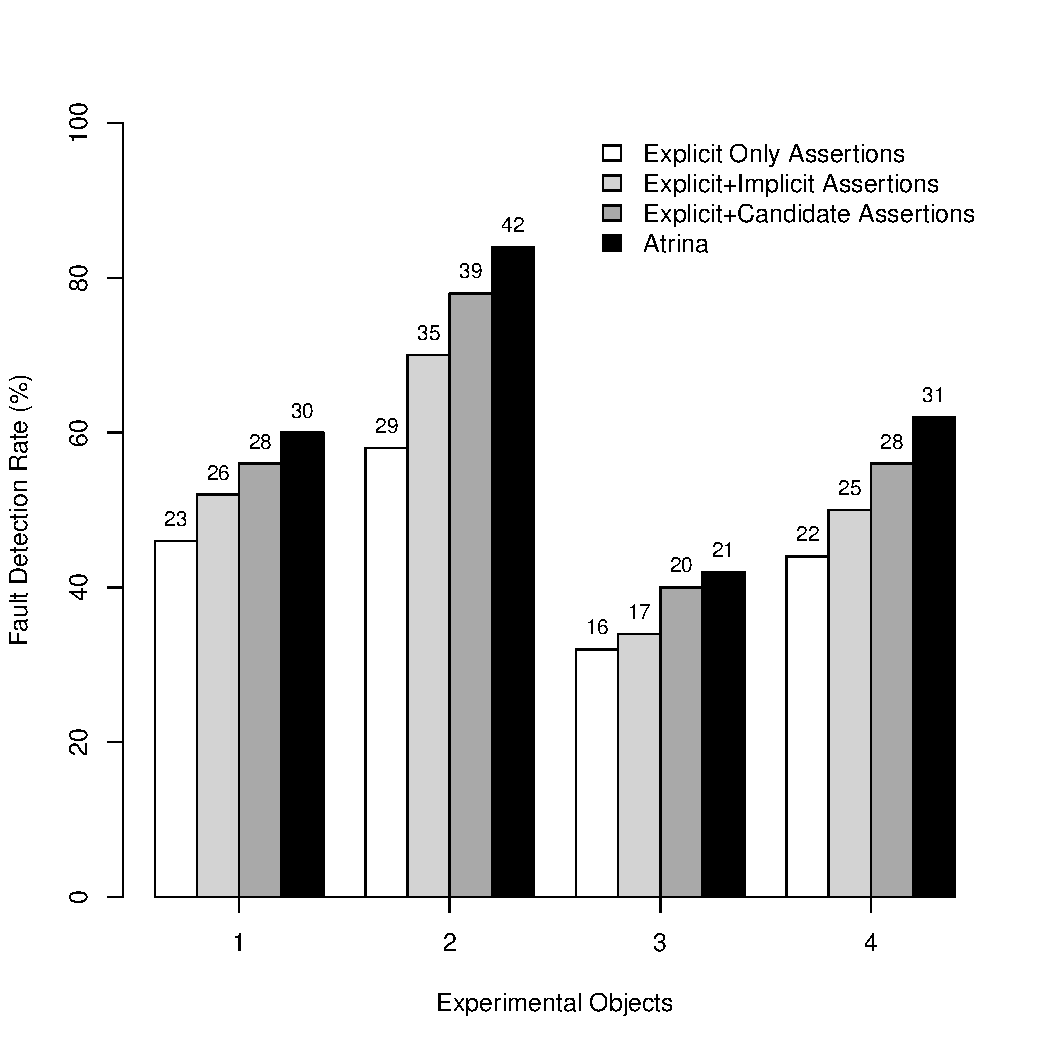
\includegraphics[width=0.8\hsize]{r-scripts/assertionTypeFaultDetec}
  \vspace{-0.18in} 
  \mycaption{Fault detection rate using different types of generated assertions.}
  \vspace{-0.3in} 
  \label{Fig:assertionTypeFaultDetec} 
\end{figure}

\headbf{Effectiveness (RQ2)} \figref{assertionTypeFaultDetec} depicts the fault detection rate (percentages) achieved by (1) \tool, (2) explicit assertions when included individually, and (3) explicit assertions in conjunction with either implicit assertions or (4) candidate assertions. The number on each bar represent the number of faults detected by the corresponding assertion types. As shown in \figref{assertionTypeFaultDetec}, \tool detects on average 62\% of the total faults (ranges from 42-84\%).
The percentage of faults detected by explicit assertions alone is less than that detected through the combination of explicit with either implicit assertions or candidate assertions. This indicates that implicit as well as candidate assertions are essential entities in improving the fault finding capability of \tool. By eliminating implicit and candidate assertions, fault detection rate drops 27\% on average, with a maximum drop of 31\% for the EnterpriseStore application (ID 2).

\figref{assertionTypeFaultDetec} shows that the improvement contributed by implicit assertions is 8\% on average, while the improvement due to candidate assertions is 21\% on average. This indicates that candidate assertions play a more prominent role in increasing the number of faults detected by \tool than implicit assertions. Not surprisingly, explicit assertions contribute the most among the three assertion types generated by \tool. Explicit assertions detect 73\% of the total faults on average (ranges from 69-77\%). These assertions are derived directly from the DOM-based oracles written by the developer of the application who has a deep knowledge of the application's behaviour. Therefore, it is not surprising that explicit assertions derived directly from such oracles have the highest impact on fault finding capability of our tool.        

\headbf{Comparison with human-written DOM-based Assertions (RQ3)}
\begin{figure}[!t]
  \centering
  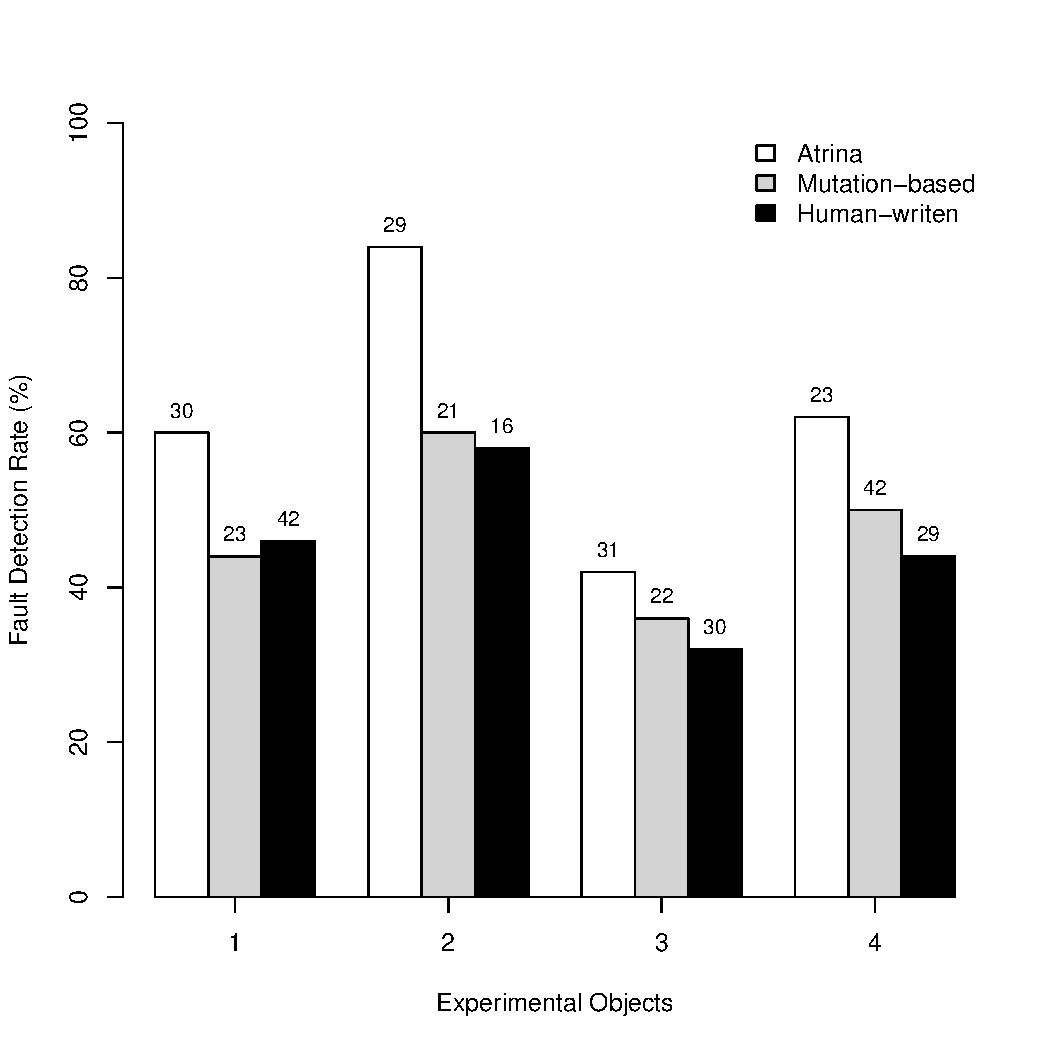
\includegraphics[width=0.8\hsize]{r-scripts/barplot-faultDetectionRate}
  \vspace{-0.18in}   
  \mycaption{Fault finding capability.}
  \vspace{-0.3in} 
  \label{Fig:barplot-faultDetectionRate}
\end{figure}
\figref{barplot-faultDetectionRate} compares the fault detection rate achieved by the code-level assertions generated by \tool with the human-written DOM-based assertions. The numbers shown on each bar represent the actual number of faults detected by the corresponding assertion generation technique. As shown in the figure, the percentage of faults found by \tool is higher than manually written DOM-based assertions for all applications. Overall, \tool outperforms manual assertions in terms of fault finding capability by 37\% on average (ranges from 30-45\%). We observed that on average, 52\% of the candidate DOM properties that we select to construct our candidate assertions were ignored in human-written DOM assertions, although their values are updated through the \javascript code.
We further noticed that for each failed manual DOM assertion as a result of an injected fault, at least one explicit assertion fails in \tool (three failed explicit assertions on average).
%This indicates that exploiting the available knowledge of the tester in the written DOM oracles can help to produce fruitful set of code-level assertions.
We observed that most often DOM assertions written by the tester are too generic in nature. Therefore even when a DOM assertion detects a \javascript fault, pinpointing the root cause of the error can be quite challenging. However, code-level assertions make it easier for the tester to localize the fault, as their locations directly correlate with the code.

We observed in several cases that the value of a DOM element property that is checked in the human-written test suite is later used in \javascript code that involves internal computations only. If the seeded fault falls in the corresponding computational statements, the resulting error is not captured through the manually written DOM assertions. In such cases, implicit assertions are capable of detecting the error, which points to the importance of incorporating these types of assertions in our approach. We also noticed that around 33\% of the faults found by implicit assertions are undetected by the human-written ones. This is because they require executing a more complex sequence of events to propagate to the observable DOM (e.g., when an object's property is assigned in a function to be later used in updating a value of a DOM element after a specific event is triggered). 

\headbf{Comparison with Mutation-based Assertion Generation (RQ4)}
\figref{barplot-faultDetectionRate} presents the results of comparing fault finding capability of \tool with mutation-based assertion generation technique. As shown in the figure, \tool produces unit assertions that are more effective than those produced by mutation-based technique in terms of fault-finding capability. The assertions generated by \tool surpasses those generated by the mutation-based approach by 29\% on average (ranges from 17-40\%), although both implementation and evaluation of the mutation-based technique use a common set of mutation operators (and thus our evaluation is biased towards mutation-based techniques).
%, which favours mutation-based assertion generation as we discussed in \secref{setup}. 
This points to the importance of incorporating the information that exists in human-written DOM-based test cases.       

While the results demonstrate that \tool is more effective than mutation-based approach in terms of fault detection, we further investigate efficiency of our approach in terms of time overhead. 
We compute overhead of \tool as the summation of time required for (1) instrumenting the application, and (2) analyzing the collected trace to compute \javascript slices. To calculate time overhead of the mutation-based approach, we consider the total time required for running the test suite multiple times (once per mutation), generating mutants, as well as the time needed to compare the original and the mutated version of the application to generate assertions. \figref{performance} shows the results of time overhead computed for each approach.    
Our results show that the time overhead for \tool is 52 seconds on average, while the overhead computed for mutation-based technique is 123 seconds on average. As shown in the figure, for the EnterpriseStore application (ID 2), which is the largest application we considered (57K LOC), time efficiency is increased by 58\% using \tool. This indicates that our approach significantly outperforms mutation-based assertion generation as far as time efficiency is concerned. 
